\documentclass{beamer}

\usepackage[utf8]{inputenc}
\usepackage[ngerman]{babel}

\usetheme{Frankfurt}
\useoutertheme[subsection=false]{miniframes}
\usepackage{color,graphicx,overpic,tikz}
\definecolor{DarkBlue}{rgb}{0.098,0.098,0.349} % RGB(25, 25, 89)
\setbeamercolor{section in head/foot}{fg=white, bg=DarkBlue}
\definecolor{LighterBlue}{rgb}{0.15,0.2,0.8}
\setbeamercolor{frametitle}{bg=LighterBlue, fg=white}
\setbeamercolor{title}{fg=white, bg=LighterBlue}
\setbeamercolor{structure}{fg=LighterBlue, bg=white}
\setbeamertemplate{headline}{}

\definecolor{LightBlue}{rgb}{0.5,0.65,1}

\newcommand{\E}{\mathbb{E}} % Euklidischer Raum
\newcommand{\R}{\mathbb{R}} % Reelle Zahlen
\newcommand{\HH}{\mathbb{H}} % Hyperbolischer Raum
\newcommand{\Bild}{\mathrm{Bild}} % Bild
\newcommand{\fa}[1]{\forall \, {#1} \,:\,} % Schöner Allquantor
\newcommand{\ex}[1]{\exists \, {#1} \,:\,} % Schöner Existenzquantor
\newcommand{\dist}{\mathsf{dist}} % Distanz

% Platzhalter
\newcommand{\blank}{\text{--}}

% Absolutwert, Norm
% siehe http://tex.stackexchange.com/questions/43008/absolute-value-symbols
\usepackage{mathtools}
\DeclarePairedDelimiter\norm{\lVert}{\rVert}
\DeclarePairedDelimiter\abs{\lvert}{\rvert}%

\theoremstyle{definition}

\newtheorem*{bspe}{Beispiele}
\newtheorem*{satz}{Satz}
\newtheorem*{lem}{Lemma}
\newtheorem*{bem}{Bemerkung}
\newtheorem*{kor}{Korollar}
\newtheorem*{prop}{Proposition}

% copied from http://tex.stackexchange.com/questions/11954/automatically-scale-big-and-small-graphics-for-beamer-presentations
\newcommand{\framedgraphic}[1] {
  \begin{frame}
    \begin{center}
      \vspace{-10pt}
      \includegraphics[width=\textwidth,height=0.85\textheight,keepaspectratio]{#1}
    \end{center}
  \end{frame}
}

\title{Alexandrov-Krümmung, Hadamard-Räume und der Satz von Cartan-Hadamard}
\author{Tim Baumann}
\institute{Seminar Metrische Geometrie}
\date{27. Mai 2014}

\begin{document}

\setlength{\abovedisplayskip}{2pt}
\setlength{\belowdisplayskip}{2pt}
\setlength{\abovedisplayshortskip}{2pt}
\setlength{\belowdisplayshortskip}{2pt}

\begin{frame}[plain]
  \titlepage
\end{frame}

\begin{frame}
  \frametitle{Krümmung in der Differentialgeometrie}

  \begin{picture}(320,150)
    \put(80,30){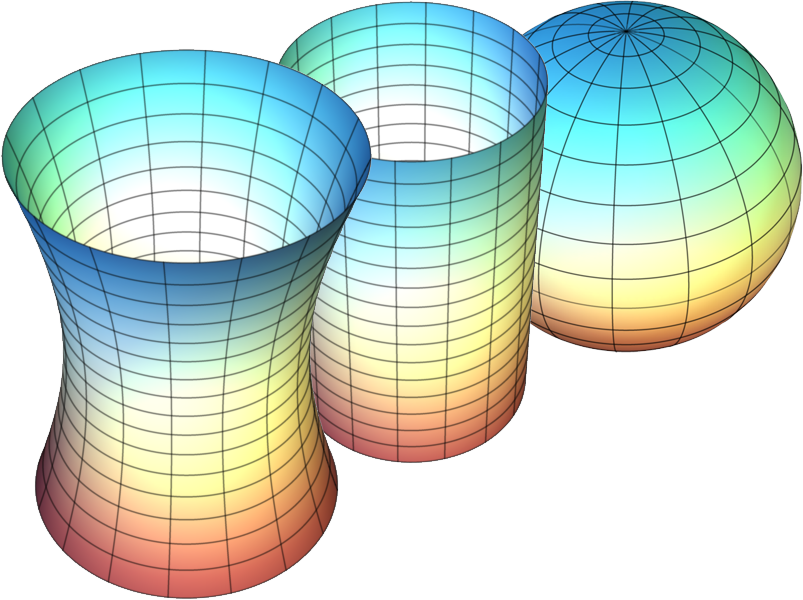
\includegraphics[scale=0.2]{bilder/Gaussian_curvature.png}}
    \put(100,15){$K < 0$}
    \put(155,40){$K = 0$}
    \put(200,65){$K > 0$}
  \end{picture}

  Für die Gaußkrümmung $K$ im Punkt $u$ gilt
  $K = \kappa_1 \cdot \kappa_2 = \det(W_u)$,
  wobei $\kappa_1$ und $\kappa_2$ die Hauptkrümmungen und
  \[ W_u := D_u \nu \circ (D_u X)^-1 : T_u X \to T_u X \]
  die Weingartenabbildung in $u$ bezeichnet.
\end{frame}

\framedgraphic{bilder/Torus_Positive_and_negative_curvature.png}

\begin{frame}
  \begin{picture}(320,100)
    \put(-20,10){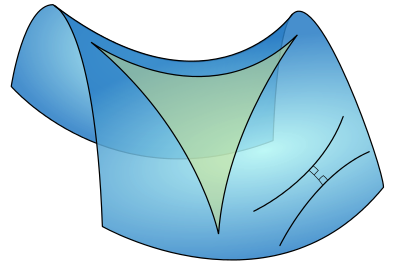
\includegraphics[scale=0.3]{bilder/400px-Hyperbolic_triangle.png}}
    \put(110,20){
      \begin{tikzpicture}
        \draw[thick,fill=LightBlue] (0,0) -- (3,0) -- (1.5,2) -- cycle;
      \end{tikzpicture}
    }
    \put(220,0){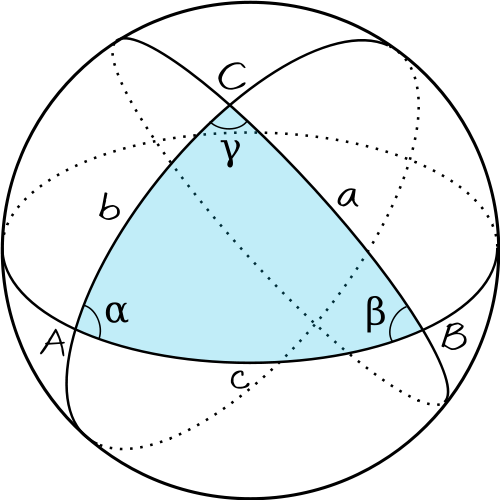
\includegraphics[scale=0.2]{bilder/500px-Triangle_spherique.png}}
    \put(35,-20){$K < 0$}
    \put(140,-20){$K = 0$}
    \put(255,-20){$K > 0$}
  \end{picture}
\end{frame}

\framedgraphic{bilder/sline-sm.jpg}
\framedgraphic{bilder/line2-ed.jpg}
\framedgraphic{bilder/line3-sm.jpg}
\framedgraphic{bilder/line4-sm.jpg}

\begin{frame}
  Für $K \in \R$ ist der Modellraum $M_K^2$ definiert durch

  \begin{align*}
    M_K^2 \coloneqq \begin{cases}
      (S^2, \tfrac{1}{\sqrt{K}} d_{S_2}) & \text{für $K > 0$,}\\
      (\E^2, d_{\E^2}) & \text{für $K = 0$,}\\
      (\HH^2, \tfrac{1}{\sqrt{-K}} d_{\HH^2}) & \text{für $K < 0$,}
    \end{cases}
  \end{align*}

  wobei $\E^2 = \R^2$ den gewöhnlichen euklidischen Raum und $\HH^2$ den zweidimensionalen hyperbolischen Raum mit konstanter Krümmung -1 bezeichnet.

  Dabei sind $d_{S^2}$ und $d_{\HH^2}$ die induzierten intrinsichen Normen.

  Im Fall $K \not= 0$ bezeichnet $\tfrac{1}{\sqrt{\abs{K}}} d$ die skalierte Metrik
  \[ (x, y) \mapsto \tfrac{1}{\sqrt{\abs{K}}} d(x, y). \]
\end{frame}

% TODO: Vergleichsdreiecke

\begin{frame}
  Sei $K \in \R$ und $(X, d)$ ein Längenraum.

  \begin{definition}
    Ein \emph{Dreieck} $\Delta abc$ in $X$ besteht aus drei Eckpunkten $a, b, c \in X$ und verbindenden kürzesten Wegen $\sigma_{ab}, \sigma_{bc}, \sigma_{ac} : \left[0,1\right] \to X$.
  \end{definition}

  \begin{definition}<2->
    Ein \emph{Vergleichsdreieck} $\Delta \overline{abc}$ von $\Delta abc$ in $M_K^2$ besteht aus drei Punkten $\overline{a}, \overline{b}, \overline{c} \in M_K^2$ und verbindenden kürzesten Wegen $\sigma_{\overline{ab}}, \sigma_{\overline{bc}}, \sigma_{\overline{ca}} : \left[0,1\right] \to M_K^2$, sodass gilt:
    \[
      d_{M_K^2}(\overline{a}, \overline{b}) = d(a, b),
      \quad
      d_{M_K^2}(\overline{b}, \overline{c}) = d(b, c),
      \quad
      d_{M_K^2}(\overline{c}, \overline{a}) = d(c, a)
    \]
  \end{definition}

  \begin{definition}<3->
    Ein Vergleichspunkt von $d \in \Bild(\sigma_{ac})$ in einem Vergleichsdreieck $\Delta \overline{abc}$ ist ein Punkt $\overline{d} \in \Bild(\sigma_{\overline{ac}})$ mit $d(a, d) = d_{M_K^2}(\overline{a}, \overline{d})$.
  \end{definition}
\end{frame}

\begin{frame}
  Sei $K \in \R$ und $(X, d)$ ein Längenraum.

  \begin{definition}
    Eine Teilmenge $U \subseteq X$ heißt \emph{CAT($K$)-Gebiet}, falls gilt:
    \begin{itemize}
      \item Für alle $x, y \in U$ gibt es eine Geodäte $\sigma_{xy} : \left[0,1\right] \to U$ der Länge $d(x, y)$.
      \item Alle Dreiecke $\Delta abc$ mit Eckpunkten und Seiten in $U$ erfüllen die CAT($K$)-Vergleichseigenschaft:\\
      Für alle $d \in \Bild(\sigma_{ac})$ mit Vergleichspunkt $\overline{d}$ in $\Delta \overline{abc}$ gilt
      \[ d(b, d) \leq d_{M_K^2}(\overline{b}, \overline{d}). \]
      und analog für $d' \in \sigma_{ab}$, $d'' \in \sigma_{bc}$.
    \end{itemize}
  \end{definition}

  \begin{definition}<2->
    Der Längenraum $X$ heißt \emph{CAT($K$)-Raum}, falls $X$ eine Überdeckung mit offenen CAT($K$)-Gebieten besitzt.\\
    Man sagt auch, der Raum habe \emph{Alexandrov-Krümmung $\leq K$}.
  \end{definition}
\end{frame}

\begin{frame}
  \frametitle{Warum der Name CAT($K$)?}

  \begin{center}
    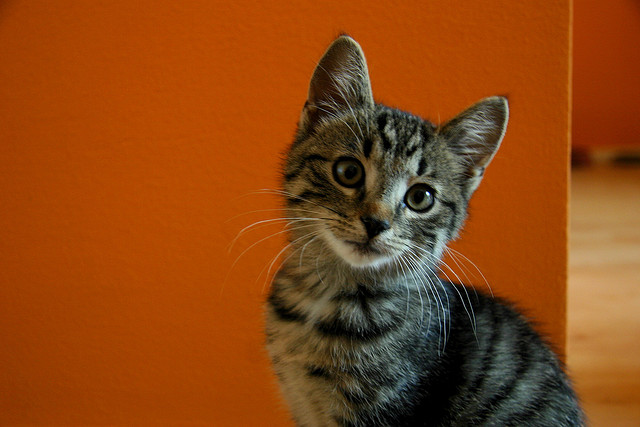
\includegraphics[scale=0.4]{bilder/cat.jpg}
  \end{center}
\end{frame}

\begin{frame}
  \footnotesize
  \begin{picture}(330,160)
    \put(-10,20){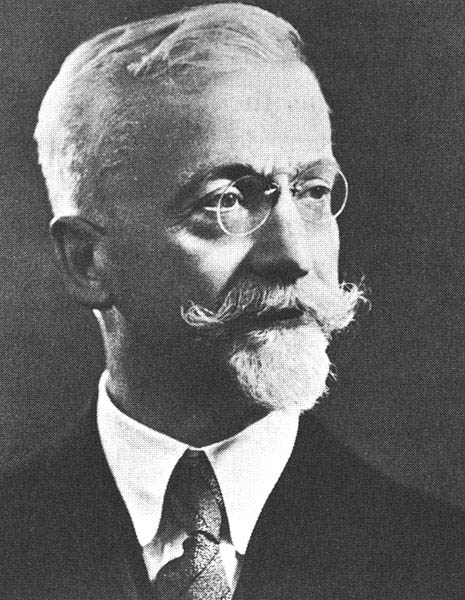
\includegraphics[height=0.5\textheight,keepaspectratio]{bilder/Elie_Cartan.jpg}}
    \put(-10,0){Élie Cartan}
    \put(-10,-10){(1869-1951)}
    \put(100,20){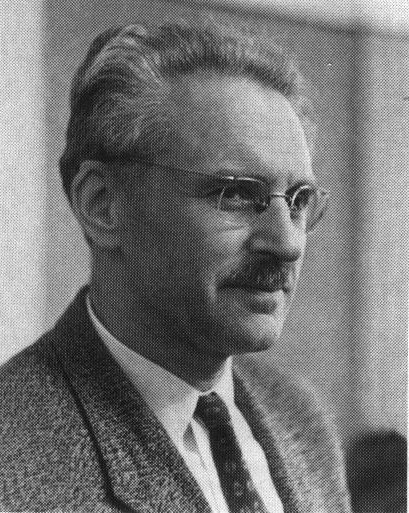
\includegraphics[height=0.5\textheight,keepaspectratio]{bilder/Aleksandr_Danilovich_Aleksandrov_1952.jpg}}
    \put(100,0){Alexander D. Alexandrov}
    \put(100,-10){(1912-1999)}
    \put(213,20){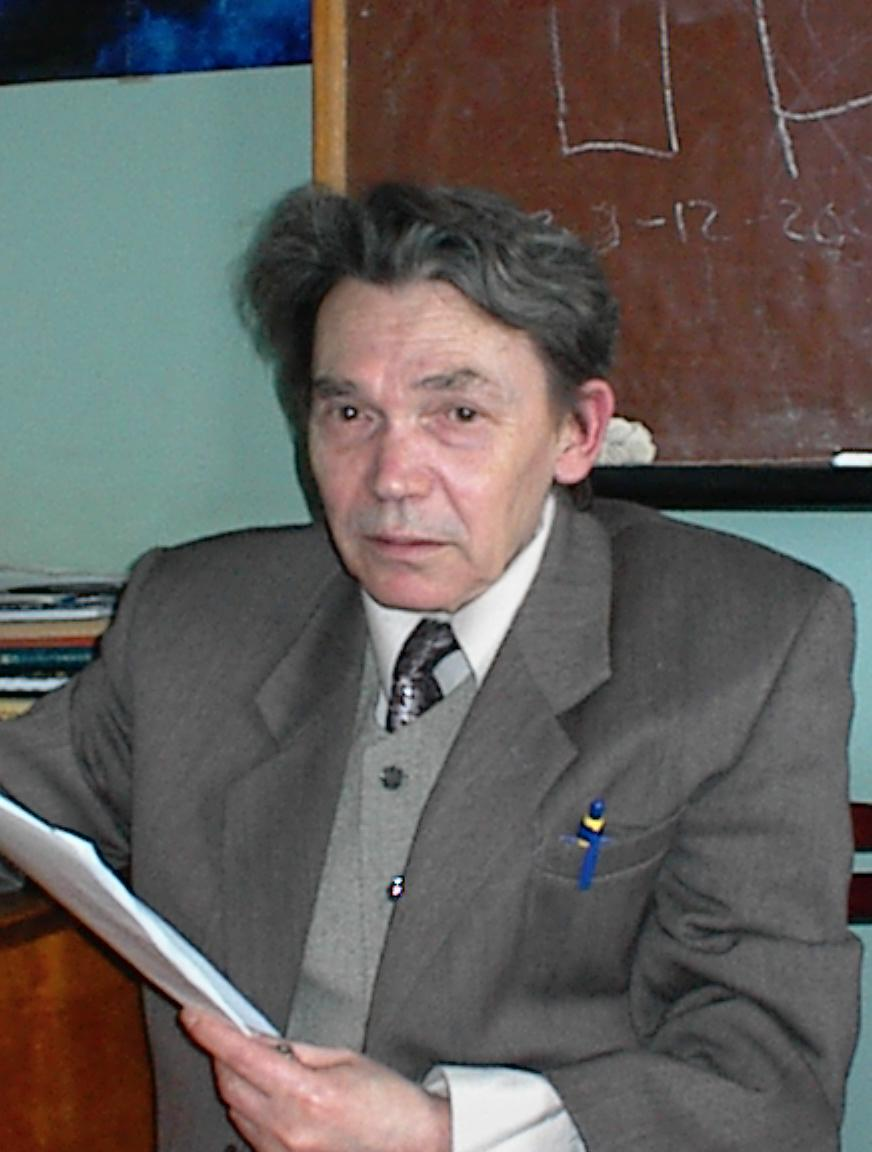
\includegraphics[height=0.5\textheight,keepaspectratio]{bilder/Toponogov.jpg}}
    \put(213,0){Victor A. Toponogov}
    \put(213,-10){(1930-2004)}
  \end{picture}
\end{frame}

\begin{frame}
  \begin{bem}[BBI, Exercise 4.1.11]
    Es reicht aus, in der Definition die Ungleichung
    \[ d(b, d) \leq d_{M_K^2}(\overline{b}, \overline{d}) \]
    nur für Mittelpunkte $d$ der Seite $\sigma_{ac}$, also $d \in \Bild(\sigma_{ac})$ mit $d(a, d) = d(d, c) = \tfrac{1}{2} d(a, c)$, zu fordern.
  \end{bem}

  \begin{bspe}<2->
    % TODO: Langsam einblenden
    \begin{itemize}
      \item<2-> $\R^n$ ist ein CAT(0)-Raum.
      \item<3-> $\R^2 \setminus B_1(0)$ ist ein CAT(0)-Raum.
      %\item Eine offene Teilmenge eines CAT($K$)-Raums ist selbst ein CAT($K$)-Raum.
      \item<4-> Klebe drei Kopien des Strahls $\left[0,\infty\right)$ am Punkt $0$ zusammen. Dieser Raum hat nichtpositive Krümmung.
    \end{itemize}
  \end{bspe}

  % Ballman, Remark 3.7 (page 15)
  \begin{satz}[Ballman, 3.7]<5->
    Sei $X$ eine Riemannsche Mannigfaltigkeit. Dann ist die Alexandrov-Krümmung von $X$ höchstens $K$ genau dann, wenn die Schnittkrümmung von $X$ nach oben durch $K$ beschränkt ist.
  \end{satz}
\end{frame}

\begin{frame}
  \begin{satz}[Kosinussatz]
    \begin{picture}(320,50)
      \put(0, 35){In jedem wie rechts beschrifteten Dreieck gilt}
      \put(50,15){$c^2 = a^2 + b^2 - 2ab \cos \gamma$}
      \put(240,0){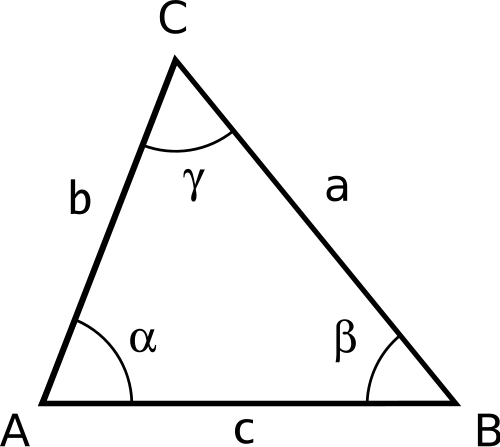
\includegraphics[scale=0.1]{bilder/500px-Triangle_-_angles,_vertices,_sides.png}}
    \end{picture}
  \end{satz}

  % BBI, p. 96
  \begin{definition}<2->
    Für drei Punkte $x, y, z$ aus einem metrischen Raum $(X, d)$ heißt
    \[ \widetilde{\measuredangle} xyz \coloneqq \arccos \frac{d(y, x)^2 + d(y, z)^2 - d(x, z)^2}{2 \cdot d(y, x) \cdot d(y, z)} \]

    \emph{Vergleichswinkel}.
  \end{definition}

  \begin{definition}<3->
    Sei $(X, d)$ ein Längenraum, $p \in X$ und $\alpha, \beta : \left[0, \epsilon\right) \to X$ zwei Geodäten mit $\alpha(0) = \beta(0) = p$. Falls der Limes existiert, so heißt
    \[ \measuredangle (\alpha, \beta) = \lim_{s,t \to 0} \widetilde{\measuredangle} (\alpha(s),p,\beta(t)) \]
    \emph{Winkel} zwischen $\alpha$ und $\beta$.
  \end{definition}
\end{frame}

\begin{frame}
  Sei $(X, d)$ ein Längenraum, $U \subseteq X$ ein CAT($0$)-Gebiet.

  \begin{prop}[BBI, 4.3.5]
    Seien $\alpha, \beta : \left[0,\epsilon\right] \to U$ kürzeste Wege mit $\alpha(0) = \beta(0) = p$.\\
    Dann ist die Abbildung
    \[ \Theta : \left[0,\epsilon\right] \times \left[0,\epsilon\right] \to \left[ 0, \pi \right], \quad (s, t) \mapsto \widetilde{\measuredangle}(\alpha(s),p,\beta(t)) \]
    monoton steigend in beiden Argumenten.
  \end{prop}

  \begin{kor}[BBI, 4.3.2]<2->
    Sei $\Delta abc$ ein Dreieck in $U$. Dann sind die Winkel
    \[
      \alpha \coloneqq \measuredangle (\sigma_{ab}, \sigma_{ac}),
      \quad
      \beta \coloneqq \measuredangle (\sigma_{ba}, \sigma_{bc}),
      \quad
      \gamma \coloneqq \measuredangle (\sigma_{ca}, \sigma_{cb}),
    \]
    wohldefiniert und es gilt $\alpha + \beta + \gamma \leq \pi$.
  \end{kor}

  % BBI, p. 4.3.5.
  \begin{bem}<3->
    Die Behauptung des Korollars ist äquivalent zur CAT($0$)-Vergleichseigenschaft, kann also auch als zur Definition von CAT($0$)-Gebieten verwendet werden.
  \end{bem}
\end{frame}

\begin{frame}
  \begin{prop}[BBI, 9.1.17]
    Sei $(X, d)$ ein Längenraum, $U = B_r(x_0) \subseteq X$ ein CAT($0$)-Gebiet. Dann gilt:
    \begin{enumerate}
      \item Für alle $a, b \in U$ gibt es einen eindeutigen kürzesten Weg, der $a$ und $b$ verbindet, und dieser ist in $U$ enthalten.
      \item Seien $\sigma_{ab}$ und $\sigma_{bc}$ zwei kürzeste Wege in $U$, die in $b$ enden bzw. starten. Falls $\measuredangle abc = \pi$, dann ist auch $\sigma_{ab} * \sigma_{bc}$ ein kürzester Weg.
      \item Jede Geodäte in $U$ ist ein kürzester Weg.
    \end{enumerate}
  \end{prop}
\end{frame}

\begin{frame}
  \begin{lem}[BBI, 9.2.3]
    Sei $(X, d)$ ein Längenraum, $U \subseteq X$ ein CAT($0$)-Gebiet und $\alpha, \beta : I \to U$ zwei durch dasselbe Intervall $I$ parametrisierte und mit jeweils konstanter Geschwindigkeit durchlaufene Geodäten in $U$. Dann ist die Distanzfunktion
    \[ \delta : I \to \R_{\geq 0}, \quad t \mapsto d(\alpha(t), \beta(t)) \]
    konvex.
  \end{lem}
\end{frame}

% Alexandrovs Lemma
% Zusammenkleben von CAT-Dreiecken
% Beispiele: Stern, $\R^2 \setminus B_1(0)$
% Definition einfach Zusammenhängend

\framedgraphic{bilder/Picture15.jpg}

\begin{frame}
  \begin{lem}[Alexandrov's Lemma]
    Seien $a, b, c, d \in \E^2$, sodass $a$ und $c$ auf verschiedenen Halbebenen bezüglich der Verbindungsstrecke $[bd]$ liegen. Seien $\tilde{a}, \tilde{b}, \tilde{c} \in \E^2$ mit
    \[
      d(a, b) = d(\tilde{a}, \tilde{b}), \quad
      d(b, c) = d(\tilde{b}, \tilde{c}), \quad
      d(a, d) + d(d, c) = d(\tilde{a}, \tilde{c}).
    \]
    Sei $\tilde{d} \in [\tilde{a}, \tilde{c}]$ mit $d(\tilde{a}, \tilde{d}) = d(a, d)$. Dann gilt:
    \begin{itemize}
      \item<1-> $\measuredangle adb + \measuredangle bdc < \pi$ genau dann, wenn $d(\tilde{b}, \tilde{d}) < d(d, b)$. Dann gilt auch $\measuredangle \tilde{b} \tilde{a} \tilde{d} < \measuredangle bad$ und $\measuredangle \tilde{b} \tilde{c} \tilde{d} < \measuredangle bcd$.
      \item<2-> $\measuredangle adb + \measuredangle bdc > \pi$ genau dann, wenn $d(\tilde{b}, \tilde{d}) > d(d, b)$. Dann gilt auch $\measuredangle \tilde{b} \tilde{a} \tilde{d} > \measuredangle bad$ und $\measuredangle \tilde{b} \tilde{c} \tilde{d} > \measuredangle bcd$.
    \end{itemize}
  \end{lem}

  \begin{lem}<3->
    Sei $(X, d)$ ein Längenraum, $\Delta abc$ ein Dreieck in $X$ und $d \in \Bild(\sigma_{ac})$. Wenn die Teildreiecke $\Delta abd$ und $\Delta cbd$ die CAT($0$)-Vergleichseigenschaft erfüllen, dann auch $\Delta abc$.
  \end{lem}
\end{frame}

\begin{frame}
  \begin{definition}
    Sei $X$ ein topologischer Raum, $\gamma_1, \gamma_2 : \left[ 0, 1 \right] \to X$ stetige Kurven mit $p = \gamma_1(0) = \gamma_2(0)$ und $q = \gamma_1(1) = \gamma_2(1)$. Eine \emph{Homotopie} zwischen $\gamma_1$ und $\gamma_2$ ist eine stetige Abbildung
    \[ H : \left[0,1\right] \times \left[0,1\right] \to X \]
    mit
    \begin{itemize}
      \item $H(\blank, 0) = \gamma_1$,
      \item $H(\blank, 1) = \gamma_2$,
      \item $H(0, t) = p$ für alle $t \in \left[0,1\right]$,
      \item $H(1, t) = q$ für alle $t \in \left[0,1\right]$.
    \end{itemize}
  \end{definition}

  \begin{definition}<2->
    Ein topologischer Raum $X$ heißt \emph{einfach zusammenhängend}, falls
    \begin{itemize}
      \item er wegzusammenhängend ist und
      \item jeder geschlossene Weg $\gamma : \left[0,1\right] \to X$ (d.\,h. $\gamma(0) = \gamma(1) =: p$) homotop zum konstanten Weg $t \mapsto p$ ist.
    \end{itemize}
  \end{definition}
\end{frame}

\end{document}